\documentclass[11pt]{article}

% --- arXiv-ready preamble (compiles with pdflatex + bibtex) -----------------
\usepackage[utf8]{inputenc}
\usepackage[T1]{fontenc}
\usepackage{lmodern}
\usepackage[margin=1in]{geometry}
\usepackage{graphicx}
\usepackage{booktabs}
\usepackage{amsmath}
\usepackage{xcolor}
\usepackage{microtype}
\usepackage[numbers,sort&compress]{natbib}
\usepackage{hyperref}
\hypersetup{colorlinks=true, linkcolor=blue!50!black, citecolor=blue!50!black, urlcolor=blue!50!black}
\graphicspath{{figures/}}

\newcommand{\pass}{\textcolor{green!55!black}{\checkmark}}
\newcommand{\fail}{\textcolor{red!75!black}{\ding{55}}}
\newcommand{\na}{\textcolor{gray}{--}}
\usepackage{pifont}

\title{\textbf{agentmem-bench: A Reproducible Benchmark for\\ Multi-Agent Memory Coordination}}
\author{Aneesh \\ \texttt{devsforfun} \\ \texttt{github.com/rooney011/agentmem-bench}}
\date{Working draft --- \today}

\begin{document}
\maketitle

\begin{abstract}
Existing agent-memory benchmarks (LoCoMo, LongMemEval) evaluate a single agent
recalling information from one long conversation. We argue this misses the dominant
failure mode of \emph{multi-agent} systems, where memory is shared and the hard
problems are coordination: contradictory writes, temporal validity, scope leakage,
concurrent-write convergence, and conflict-resolution policy. We introduce
\textbf{agentmem-bench}, a reproducible benchmark of seven deterministic scenarios
(S1--S7) that isolate these properties, and evaluate seven shipped memory systems
(AgentMem, Mem0, Zep, Cognee, Supermemory, LangMem, and a raw pgvector baseline)
behind a uniform black-box adapter, with an in-process reference implementation that
validates the scenarios themselves. We report per-scenario, per-metric results---not
a single score---and find the capability space sharply non-uniform: contradiction
detection/resolution and conflict policies are provided by exactly one system;
bitemporal ``what was true at $T$?'' retrieval by exactly one \emph{other} system;
CRDT convergence by \emph{none}, because no shipping system exposes a replica API to
a black-box test; and a raw vector store matches the managed systems on every
property that does not require coordination machinery. Beyond the grid, running the
benchmark surfaced reproducible operational failures (LLM-quota-coupled 5xx errors,
silent content deduplication that drops scope changes, ${\sim}50$\,s indexing
latencies, and a configuration in which one system enforces no isolation at all).
We release the harness, scenarios, and complete run logs, and disclose prominently
that the benchmark's authors also build one of the systems under test.
\end{abstract}

\section{Introduction}
LLM agents increasingly operate in groups---planners, executors, critics---that read
and write a shared memory. When such systems fail, it is rarely because a model
forgot a fact. Cemri et al.~\cite{cemri2025mast} construct the Multi-Agent System
Failure Taxonomy from 1{,}600+ annotated traces across seven frameworks, with
production failure rates of 41--86.7\%, and identify \emph{inter-agent misalignment}
(agents contradicting or duplicating one another's work) as one of three top-level
failure categories. Acharya~\cite{acharya2026semconsensus} reports that ${\sim}79\%$
of multi-agent failures stem from specification and coordination issues rather than
model capability. Memory is the substrate on which such coordination is resolved or
compounded.

Yet the benchmarks the field cites---LoCoMo~\cite{maharana2024locomo},
LongMemEval~\cite{wu2025longmemeval}---measure single-agent long-context recall;
Letta~\cite{letta2025locomo} argues these measure retrieval, not agentic memory.
They answer ``can the model retrieve what was said?'', not ``when two agents disagree
about the same entity, what does the system do?''. The second question is what breaks
production multi-agent apps.

We close that gap. Our contributions:
\begin{enumerate}
  \item \textbf{Seven coordination scenarios (S1--S7)} with deterministic assertions:
  contradiction detection/resolution, temporal validity, scope enforcement, CRDT
  convergence, cross-workflow isolation, policy fidelity, and an operational envelope
  (\S\ref{sec:design}).
  \item \textbf{A uniform black-box adapter} plus an in-process \textbf{reference
  implementation} that passes all scenarios, validating that the assertions are
  satisfiable; and a principled \emph{wrong-answer / unsupported (N/A) / crash}
  taxonomy (\S\ref{sec:taxonomy}).
  \item \textbf{An evaluation of seven shipped systems} under pinned models and
  committed fixtures, reported as a per-metric matrix, not a leaderboard
  (\S\ref{sec:results}).
  \item \textbf{Qualitative operational findings} the runs exposed
  (\S\ref{sec:operational}).
  \item \textbf{A fully reproducible release} with one-command runs, committed raw
  logs, and an explicit conflict-of-interest disclosure (\S\ref{sec:coi}).
\end{enumerate}

Our central claim is deliberately anti-climactic: \emph{there is no ``best''
multi-agent memory system}---capabilities are disjoint, several systems provide none
beyond a vector store, and one property (CRDT convergence) is unverifiable in every
shipping product.

\section{Related Work}
\textbf{Single-agent memory benchmarks.} LoCoMo~\cite{maharana2024locomo} and
LongMemEval~\cite{wu2025longmemeval} evaluate long-term recall in extended
single-agent dialogues; the Mem0 system paper~\cite{chhikara2025mem0} compares memory
systems on single-agent retrieval quality and cost. We complement, not replace, these
with an orthogonal multi-agent dimension. \textbf{Temporal knowledge graphs.}
Zep/Graphiti~\cite{rasmussen2025zep} maintain bitemporal facts with validity
intervals, which our S2 directly exercises. \textbf{Coordination and CRDTs.}
Cemri et al.~\cite{cemri2025mast} motivate the coordination-failure framing;
CodeCRDT~\cite{codecrdt2025} adapts convergence testing to multi-agent code editing
(we borrow its order-independence framing for S4); Semantic
Consensus~\cite{acharya2026semconsensus} informs S6's conflict-type taxonomy
(contradictory, contention-based, causally invalid). \textbf{Architectures.}
MemGPT~\cite{packer2023memgpt} frames the LLM as an operating system with paged
memory; it is representative of the systems whose coordination properties we measure.

\section{Benchmark Design}\label{sec:design}
\textbf{Principles.} Scenarios are deterministic (fixed inputs, committed fixtures),
black-box (public API only), and designed to \emph{separate} a memory system from a
vector store---hence the pgvector control: any scenario it passes is recognized as
not measuring memory-system value. A system lacking a needed API scores \emph{N/A},
never a failure.

\textbf{Adapter.} Each system implements \texttt{write}, \texttt{search}
(\texttt{at\_time} optional), and optional \texttt{check\_conflicts},
\texttt{set\_policy}, and a replica/vector-clock surface for S4. Unsupported methods
raise \texttt{Unsupported}, recorded as N/A. Adapters are ${\sim}100$ lines.

\textbf{Scenarios.}
\begin{itemize}
  \item \textbf{S1 Contradiction}: two agents write conflicting facts. Metrics:
  \emph{detected}, \emph{resolved} (under \texttt{planner\_wins}), \emph{consistent}.
  \item \textbf{S2 Temporal}: write F1 at $T_0$, contradicting F2 at $T_1$; query
  \texttt{at\_time}. Metrics: $t_0$ (returns F1), $t_1$ (returns F2), \emph{bitemporal}.
  \item \textbf{S3 Scope}: \texttt{private} then \texttt{team}; \emph{isolated},
  \emph{team\_visible}, \emph{cross\_workflow}.
  \item \textbf{S4 CRDT}: conflicting writes on two replicas, synced out-of-order;
  \emph{converge}, \emph{deterministic} (10 orders), \emph{lossless}.
  \item \textbf{S5 Isolation}: many writes across two workflows; \emph{leakage\_rate}.
  \item \textbf{S6 Policy}: \texttt{ignore} / \texttt{timestamp\_wins} /
  \texttt{planner\_wins} / \texttt{human\_in\_loop}; retrieval must match each.
  \item \textbf{S7 Operational}: write/search latency distribution and cost.
\end{itemize}

\textbf{Result taxonomy.}\label{sec:taxonomy} We distinguish \emph{wrong answer}
(assertion violated $\to$ fail), \emph{unsupported} (no such API $\to$ N/A), and
\emph{crash} (5xx/exception/timeout $\to$ re-run once). Conflating ``can't do X''
with ``did X wrong'' produces misleading leaderboards.

\textbf{Reference implementation.} An in-process \texttt{FakeSUT} implements correct
semantics for all scenarios and passes every correctness metric, validating that the
assertions are satisfiable and sound---a check absent from most benchmarks.

\section{Systems Under Test \& Setup}\label{sec:sut}
We evaluate AgentMem, Mem0, Zep, Cognee, Supermemory, LangMem, and a pgvector
baseline (INSERT + cosine top-$k$), plus the FakeSUT reference. Embeddings follow each
system's default (the out-of-box experience), documented per system; models are
pinned to version strings. The harness runs with one command per system and emits a
self-contained \texttt{runs/<id>/} directory (manifest, per-metric JSONL, latency and
cost JSON); \texttt{compare.py} merges runs into the matrix with provenance. Hosted
systems with low free-tier quotas were run at reduced operation counts for S5/S7 via
documented knobs; latency percentiles are robust to smaller $N$. Asynchronous
pipelines are awaited to index-visibility rather than slept on.

\section{Results}\label{sec:results}

\begin{figure}[t]
  \centering
  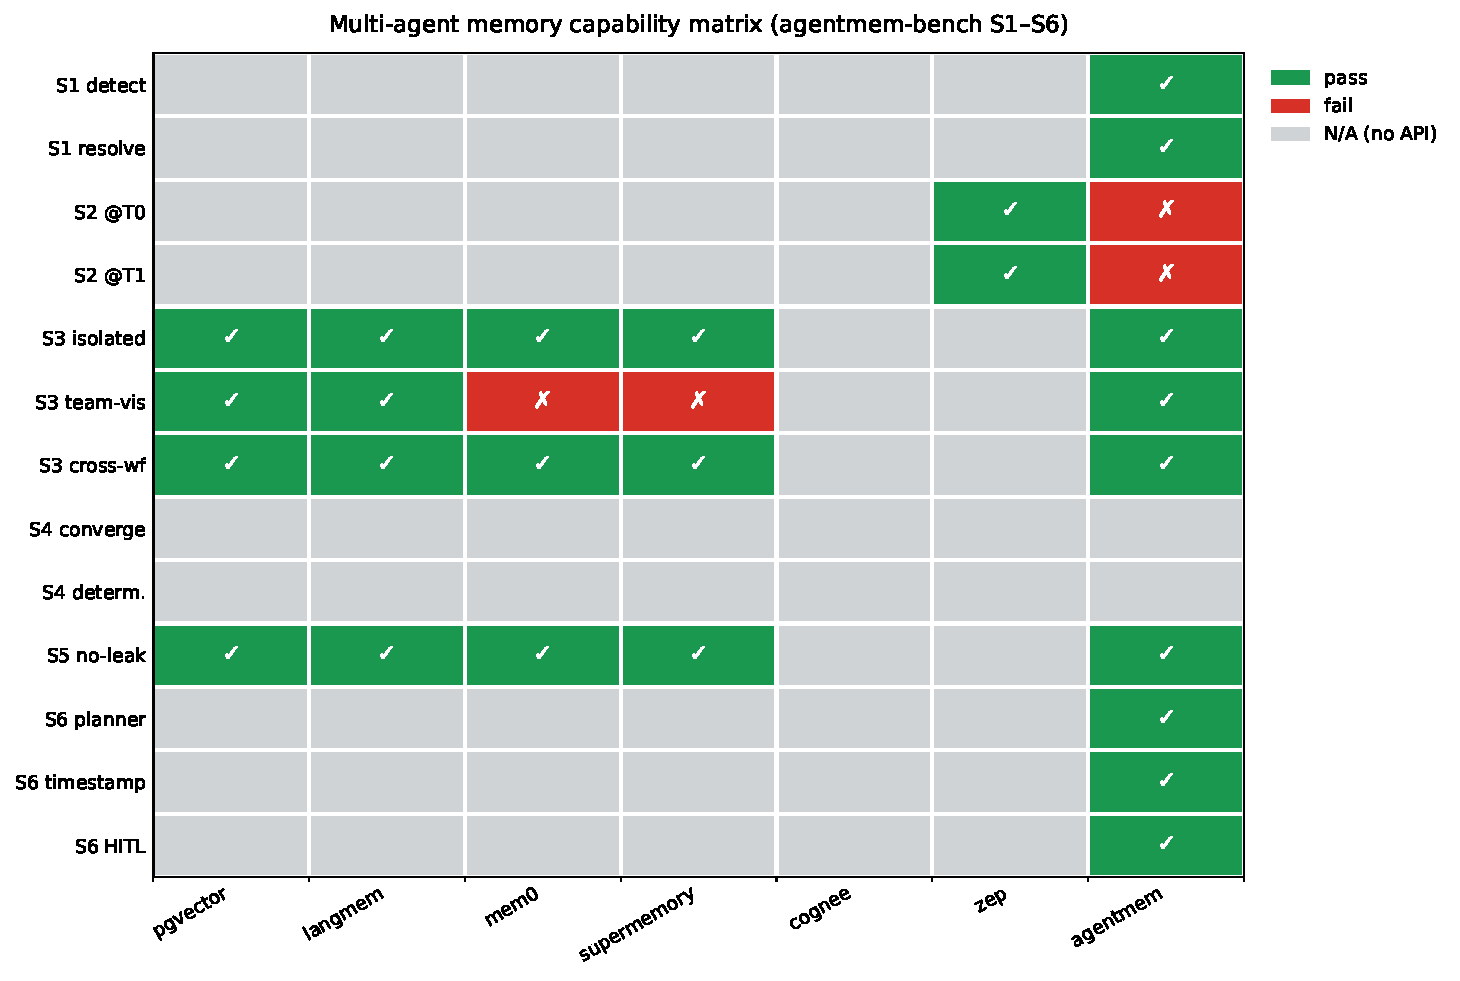
\includegraphics[width=0.92\linewidth]{capability_heatmap.pdf}
  \caption{Capability matrix across S1--S6. Green = pass, red = fail, gray = N/A (no
  API). Only AgentMem fills S1 (contradiction) and S6 (policy); only Zep fills S2
  (temporal); S4 (CRDT) is N/A for every shipping system. AgentMem's S2 failure (it
  accepts \texttt{at\_time} but returns both facts) is shown in red.}
  \label{fig:heatmap}
\end{figure}

Figure~\ref{fig:heatmap} summarizes correctness. \textbf{S1 (contradiction):} only
AgentMem exposes a conflict-detection API and resolves per policy (it blocked the
executor's conflicting write under \texttt{planner\_wins} with a high-severity
conflict description). No other system surfaces a contradiction; we verified Mem0's
write-time LLM dedup does \emph{not} resolve it---the stale and new values coexist.
\textbf{S2 (temporal):} only Zep answers point-in-time queries correctly, via
bitemporal fact invalidation ($\texttt{invalid\_at}=T_1$); AgentMem accepts
\texttt{at\_time} but returns both facts (a genuine gap), and others lack temporal
queries entirely. \textbf{S3/S5 (scope):} expressible as filter predicates, so the
baselines pass---confirming these do not differentiate memory systems from vector
stores; the informative split is intra-tier: \emph{verbatim stores (pgvector,
LangMem, AgentMem) preserve a re-scoped fact; dedup/aggregating stores (Mem0,
Supermemory) silently drop the scope change}. \textbf{S4 (CRDT):} N/A for every
shipping system---none exposes a replica/vector-clock API drivable by a black-box
convergence test; only the reference passes. \textbf{S6 (policy):} AgentMem satisfies
all four policies to spec; no other system ships conflict policies.

\begin{figure}[t]
  \centering
  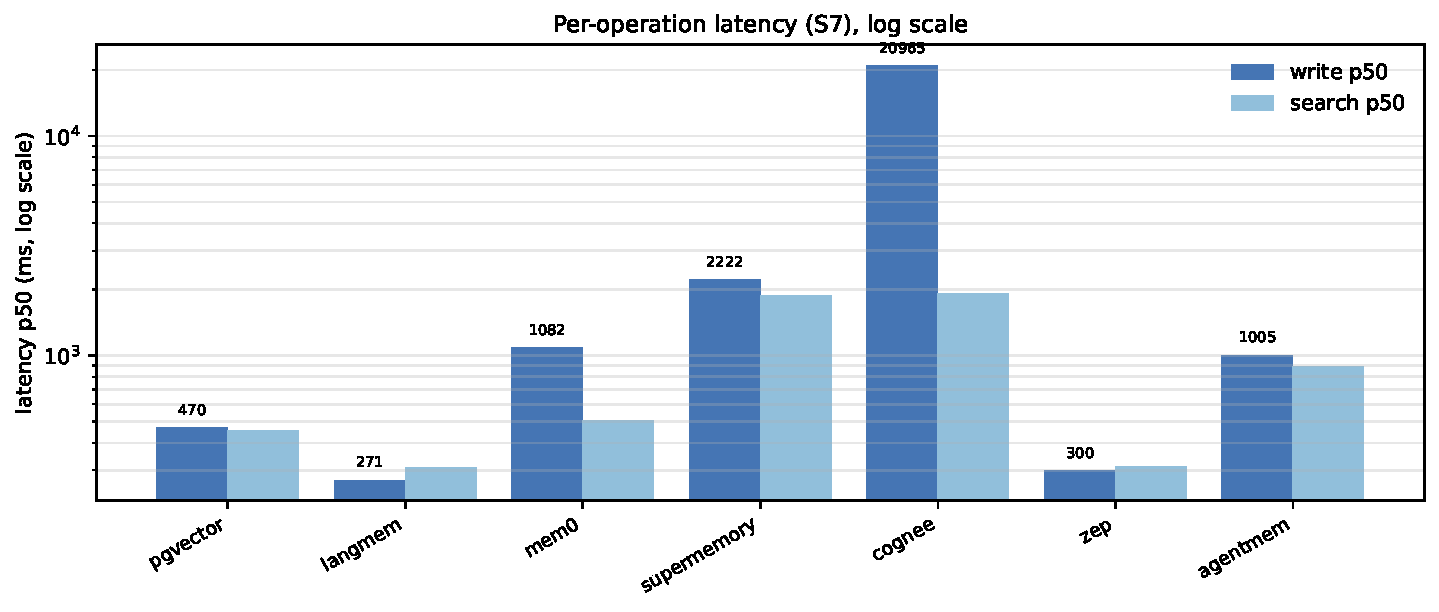
\includegraphics[width=0.92\linewidth]{latency.pdf}
  \caption{Per-operation latency (S7), $\log$ scale. A ${\sim}70\times$ spread:
  LangMem/Zep/pgvector ${\approx}300$\,ms; AgentMem/Mem0 ${\approx}1$\,s; Supermemory
  ${\approx}2.2$\,s; Cognee ${\approx}21$\,s (per-write LLM graph extraction).}
  \label{fig:latency}
\end{figure}

\textbf{S7 (operational, Table~\ref{tab:latency}).} The four quota-unconstrained
systems are reported with full per-operation distributions ($N{=}100$, or $40$ for
Mem0); the three slow/quota-limited systems retain single-run percentiles at the
stated $N$ (their order-of-magnitude latency is unambiguous regardless of $N$).

\begin{table}[t]
  \centering
  \small
  \caption{S7 write latency (ms). mean$\pm$std and percentiles over the per-op samples
  in a run. $^{\dagger}$single run at small $N$; mean/std omitted.}
  \label{tab:latency}
  \begin{tabular}{lrrrrr}
    \toprule
    System & mean$\pm$std & p50 & p95 & p99 & $N$ \\
    \midrule
    LangMem      & $319.6\pm208.4$ & 270.8 & 444.0 & 941.5 & 100 \\
    Zep          & $322.1\pm113.4$ & 299.5 & 405.4 & 767.8 & 100 \\
    pgvector     & $518.8\pm260.0$ & 469.9 & 725.3 & 1425.2 & 100 \\
    Mem0         & $1119.5\pm145.1$ & 1082.4 & 1498.4 & 1661.0 & 40 \\
    AgentMem     & \na & 1004.9 & 1084.2 & --- & ${\sim}20^{\dagger}$ \\
    Supermemory  & \na & 2221.6 & 7172.5 & --- & ${\sim}30^{\dagger}$ \\
    Cognee       & \na & 20965.4 & 28168.0 & --- & ${\sim}5^{\dagger}$ \\
    \bottomrule
  \end{tabular}
\end{table}

\section{Operational Findings}\label{sec:operational}
Static metrics understate what running the systems revealed.
\begin{itemize}
  \item \textbf{LLM-quota coupling (AgentMem).} Conflict detection/extraction is
  backed by a generative model; under a daily free-tier quota it returned \texttt{500}
  rather than degrading gracefully, and we observed a \texttt{500} under
  near-simultaneous policy writes. S6 completed only after provisioning fresh model
  quota on the backend---an honest demonstration of fragility in the authors' own
  system.
  \item \textbf{Dedup that drops scope (Mem0, Supermemory).} Re-writing identical
  content at a wider scope returns the original record's identity (Mem0) or aggregates
  to one memory (Supermemory), losing the scope change (the S3 \emph{team\_visible}
  failure).
  \item \textbf{Indexing latency and recall (Supermemory).} ${\sim}50$\,s/doc indexing;
  its free-tier search did not reliably retrieve short factual writes, so its scope
  passes largely reflect empty results and are reported as confounded.
  \item \textbf{Isolation depends on configuration (Cognee).} In its zero-setup mode
  (access control off), search queries the global graph and leaked 100\% across
  workflows; isolation requires its multi-tenant layer.
  \item \textbf{Correct-but-slow extraction (Zep).} Asynchronous (${\sim}50$\,s)
  extraction, but the only system to deliver temporal validity.
\end{itemize}

\section{Discussion}
The results refute a one-dimensional reading of ``memory system.'' Coordination
capabilities are \emph{disjoint across vendors}: contradiction handling and policy
(AgentMem), temporal validity (Zep) are each provided by one system, and several
``memory systems'' provide nothing a vector store does not. Buyers should select by
the specific coordination property their application requires---and verify the vendor
even exposes an \emph{API} for it. A raw pgvector table is a strong, cheap baseline at
modest scale; the managed premium is justified only by the coordination axes above.

\section{Threats to Validity}
\textbf{Statistical.} Correctness cells are single deterministic runs (validated by
the reference implementation); S7 uses small $N$ on quota-limited hosted systems, and
absolute latencies are environment- and tier-bound. \textbf{Construct.} Several
systems store no scope label, so scope is emulated in the adapter; S3/S5 partly
measure the adapter (marked). \textbf{Coverage.} S4 is untestable as a black box for
all hosted systems, so CRDT is \emph{unmeasured}, not failed. \textbf{Free-tier
artifacts.} Quotas, indexing lag, and search recall on free tiers may differ from paid
deployments. \textbf{Versioning.} Hosted backends may change server-side behavior we
cannot pin; we pin client/package versions and re-publish on a cadence.

\section{Conflict of Interest}\label{sec:coi}
The authors develop \textbf{AgentMem}, one of the seven systems under test, and
AgentMem attains the only passes on S1 and S6. We mitigate as follows: (i)~this
statement is prominent; (ii)~we report AgentMem's \emph{gap} (S2) and the dimension on
which it is \emph{untestable like everyone else} (S4) in the same figure; (iii)~we
document an operational failure in our own system (\S\ref{sec:operational}); (iv)~every
scenario is a public, deterministic script and every result links to a raw trial log,
so any reader can reproduce or refute; (v)~adapters are open to PRs from competing
vendors. We report no single aggregate score.

\section{Conclusion \& Future Work}
agentmem-bench reframes memory evaluation from single-agent recall to multi-agent
coordination, and finds the capability landscape sharply differentiated and, on one
axis (CRDT), uniformly unverifiable in shipping products. v0.2 will add a
replica/vector-clock test hook so S4 can score systems that expose one, tighten
per-operation cost instrumentation, increase $N$ with seeds for confidence intervals,
and add an adversarial (prompt-injection-via-memory) scenario. We invite the community
to run the harness, contribute adapters, and challenge the methodology.

\bibliographystyle{plainnat}
\bibliography{refs}

\end{document}
